\documentclass[../main.tex]{subfiles}
\graphicspath{{\subfix{../figures/}}}
\begin{document}

The theory of quantum mechanics developed in the last century has been proved to be extremely successful in describing nature at the small scale. Typical systems treated by standard quantum mechanics are nuclei, atoms, and other systems which can be assumed to be isolated from the environment. In such systems, the Hamiltonian is postulated to be Hermitian, guaranteeing that energies are real-valued and that probabilities are conserved throughout the evolution of the system. However, in many systems, there is significant dissipation into and out of the system, and hence cannot accurately be described by standard quantum mechanics (what systems?). One way to handle such open systems is to loosen the requirement of the Hermiticity of the Hamiltonian. The resulting field of non-Hermitian quantum physics has successfully been describing systems in nuclear, atomic and optical physics in recent decades~\cite{nonHermrev}. One property of particular interest in non-Hermitian operators is the possibility of exceptional points (EPs). These correspond to points in parameter space where two or more eigenvalues and their corresponding eigenvectors of the operator simultaneously coalesce. Exceptional points have been proposed to have several useful technological applications, and along with the optical microring experiments in 2017, exceptional point sensors successfully increased the sensitivity of current and nano-particle detection~\cite{microring1, microring2}.

A different framework which treats open systems is quantum master equations, where the dynamics of the system is captured by the Liouvillian superoperator. Similarly to the Hamiltonian in non-Hermitian physics, the Liouvillian is not Hermitian due to the coupling to the environment. This brings the possibility of exceptional points also in the Liouvillian superoperator. EPs in Liouvillian physics have been of particular theoretical interest recently, and is proposed to have important applications in control and sensing technologies. Two recent examples include Ref.~\cite{thermal}, where critical decay towards the steady state in a quantum thermal machine was found at the EP; and in Ref.~\cite{steering} where an EP corresponded to optimal steering toward a target quantum state. 

An application of particular interest for quantum master equations and Liouvillian physics is electron transport in systems of quantum dots connected to metallic leads~\cite{qdottrans}. A quantum dot is a fabricated semiconductor structure containing a small number of electrons and is typically in the order of 100 nanometres in size~\cite{qdotmarcus}. The size of the dot needs to be small in comparison with the thermal wavelength of the electrons, which is why experiments are generally realized at temperatures close to absolute zero~\cite{transport}. One method of creating this tiny isolation of electrons is to apply voltages via nanoscale electrodes, called gates, which depletes the number of electrons in a small region, see \cref{fig:sem}. If the voltages are tuned successfully, the quantum dot can be tunnel coupled to the two surrounding conducting regions of the semiconductor, known as the source and drain. The electrons can then tunnel from the source into the dot and then exiting it by tunneling into the drain, producing a current through the system~\cite{qdotmarcus}. This process is schematically presented in \cref{fig:qdotscheme}.

\begin{figure}[H]
\centering
\begin{subfigure}[t]{.5\textwidth}
  \centering
  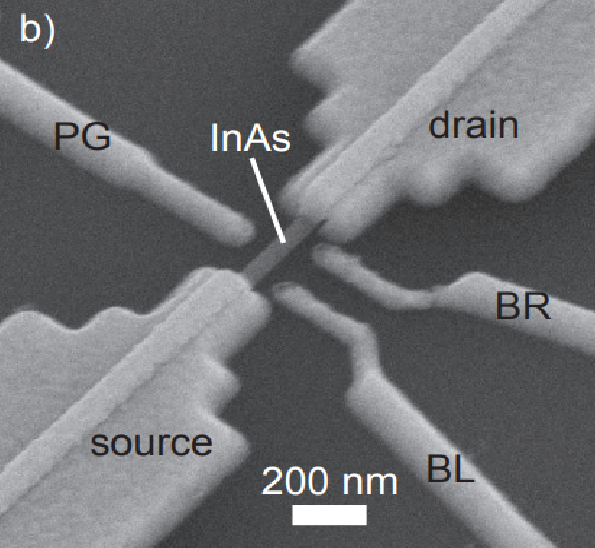
\includegraphics[width=.8\linewidth]{figures/qdotsem.png}
  \caption{}
  \label{fig:sem}
\end{subfigure}%
\begin{subfigure}[t]{.5\textwidth}
  \centering
  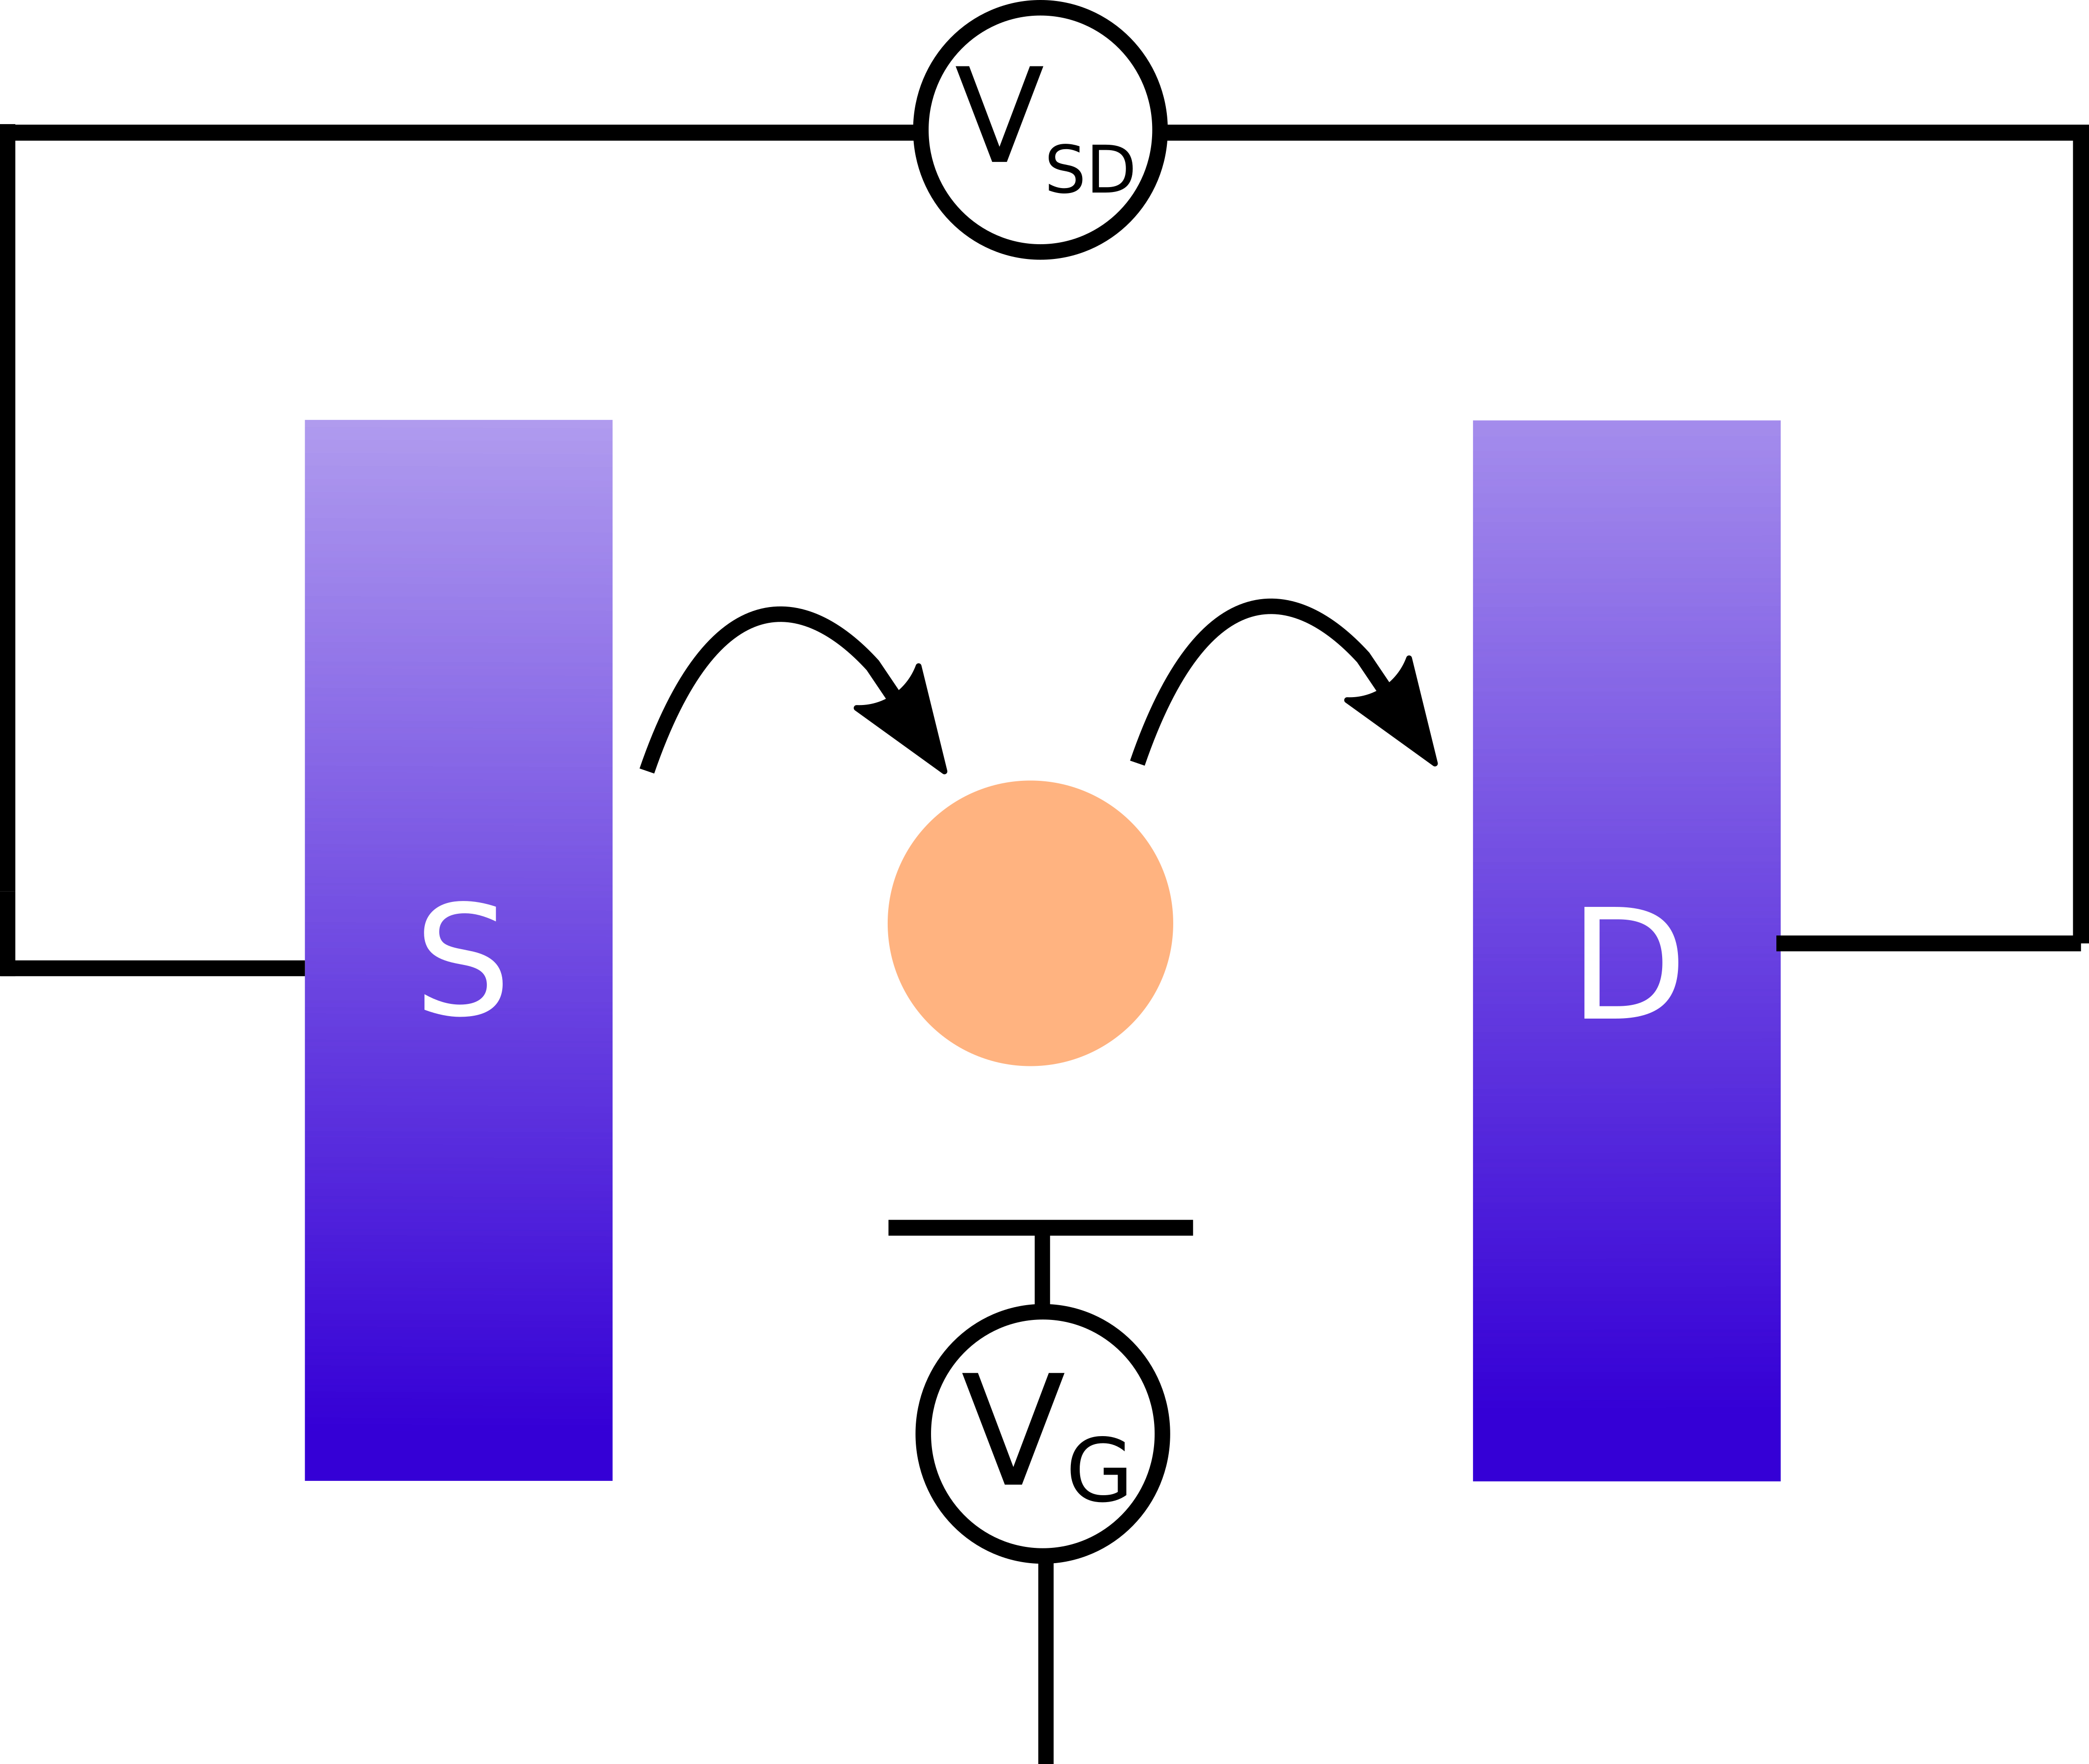
\includegraphics[width=.9\linewidth]{figures/qdotschematic.png}
  \caption{}
  \label{fig:qdotscheme}
\end{subfigure}
\caption{a) A physical implementation of a single quantum dot system. The quantum dot, labeled with InAs, the source and drain, and the gates (BR, BL and PG) are all clearly visible in this figure, captured by a scanning tunneling microscope. The figure is taken from Ref.~\cite{sven}. b) A schematic figure of a quantum dot system where the quantum dot is in the center, tunnel coupled to the source (S) and drain (D). The gate voltage $V_\text{G}$ and the source-drain voltage $V_\text{SD}$, are tuned to define the quantum dot.}
\label{fig:qdot}
\end{figure}

The wide tunability of the optical, electrical and chemical properties of quantum dots has made them useful in a large span of applications. These range from energy harvesting, display technologies, and sensors to medical and biological applications (Source). The transport set-up given in \cref{fig:qdot} in particular, has been used as a single-electron transistor

Write about QD transport and why it is interesting. Sensing. However, exceptional point physics in QDs has not been investigated very much. In this thesis, we study a quantum dot system consisting of two quantum dots coupled in parallel to metallic leads. 2nd order EP.

In this thesis, we study non-equilibrium transport properties of a parallel quantum dot system, with focus on the transient current. In particular, the dynamics at a second order EP is evaluated and understood using a combination of numerical and analytical approaches. Inspired by Ref.~\cite{thermal} and its study of EPs in thermal machines, the main purpose of the thesis is to see if similar results are visible in quantum dot systems. %Considering the sparse amount of literature on EPs in Liouvillian physics, and especially in quantum dot systems, this is (something).

The thesis is divided in the following chapters: in 

\end{document}

